%%%%%%%%%%%%%%%%%%%%%%%%%%%%%%%%%%%%%%%%%
% Short Sectioned Assignment LaTeX Template Version 1.0 (5/5/12)
% This template has been downloaded from: http://www.LaTeXTemplates.com
% Original author:  Frits Wenneker (http://www.howtotex.com)
% License: CC BY-NC-SA 3.0 (http://creativecommons.org/licenses/by-nc-sa/3.0/)
%%%%%%%%%%%%%%%%%%%%%%%%%%%%%%%%%%%%%%%%%

%----------------------------------------------------------------------------------------
%	PACKAGES AND OTHER DOCUMENT CONFIGURATIONS
%----------------------------------------------------------------------------------------

\documentclass[paper=a4, fontsize=11pt]{scrartcl} % A4 paper and 11pt font size

% ---- Entrada y salida de texto -----

\usepackage[T1]{fontenc} % Use 8-bit encoding that has 256 glyphs
\usepackage[utf8]{inputenc}
%\usepackage{fourier} % Use the Adobe Utopia font for the document - comment this line to return to the LaTeX default

% ---- Idioma --------

\usepackage[spanish, es-tabla]{babel} % Selecciona el español para palabras introducidas automáticamente, p.ej. "septiembre" en la fecha y especifica que se use la palabra Tabla en vez de Cuadro

% ---- Otros paquetes ----

\usepackage{url} % ,href} %para incluir URLs e hipervínculos dentro del texto (aunque hay que instalar href)
\usepackage{amsmath,amsfonts,amsthm} % Math packages
%\usepackage{graphics,graphicx, floatrow} %para incluir imágenes y notas en las imágenes
\usepackage{graphics,graphicx, float} %para incluir imágenes y colocarlas
\usepackage{epstopdf}

% Para hacer tablas comlejas
%\usepackage{multirow}
%\usepackage{threeparttable}

%\usepackage{sectsty} % Allows customizing section commands
%\allsectionsfont{\centering \normalfont\scshape} % Make all sections centered, the default font and small caps

\usepackage{fancyhdr} % Custom headers and footers
\pagestyle{fancyplain} % Makes all pages in the document conform to the custom headers and footers
\fancyhead{} % No page header - if you want one, create it in the same way as the footers below
\fancyfoot[L]{} % Empty left footer
\fancyfoot[C]{} % Empty center footer
\fancyfoot[R]{\thepage} % Page numbering for right footer
\renewcommand{\headrulewidth}{0pt} % Remove header underlines
\renewcommand{\footrulewidth}{0pt} % Remove footer underlines
\setlength{\headheight}{13.6pt} % Customize the height of the header

\numberwithin{equation}{section} % Number equations within sections (i.e. 1.1, 1.2, 2.1, 2.2 instead of 1, 2, 3, 4)
\numberwithin{figure}{section} % Number figures within sections (i.e. 1.1, 1.2, 2.1, 2.2 instead of 1, 2, 3, 4)
\numberwithin{table}{section} % Number tables within sections (i.e. 1.1, 1.2, 2.1, 2.2 instead of 1, 2, 3, 4)

\setlength\parindent{0pt} % Removes all indentation from paragraphs - comment this line for an assignment with lots of text

\newcommand{\horrule}[1]{\rule{\linewidth}{#1}} % Create horizontal rule command with 1 argument of height


%----------------------------------------------------------------------------------------
%	TÍTULO Y DATOS DEL ALUMNO
%----------------------------------------------------------------------------------------

\title{	
\normalfont \normalsize 
\textsc{\textbf{Curso 2016-2017} \\ Grado en Ingeniería Informática \\ Universidad de Granada} \\ [25pt] % Your university, school and/or department name(s)
\horrule{0.5pt} \\[0.4cm] % Thin top horizontal rule
\huge Práctica final: \\ Sistema experto sobre cuestiones legales y software. \\ % The assignment title
\horrule{2pt} \\[0.5cm] % Thick bottom horizontal rule
}

\author{Carlos Manuel Sequí Sánchez \\ DNI: 20 48 69 26 K} % Nombre y apellidos

\date{\normalsize\today} % Incluye la fecha actual

%----------------------------------------------------------------------------------------
% DOCUMENTO
%----------------------------------------------------------------------------------------

\begin{document}

\maketitle % Muestra el Título

\newpage %inserta un salto de página

\tableofcontents % para generar el índice de contenidos



\newpage

\section{Resumen del funcionamiento del sistema experto}
La función a desempeñar por el sistema experto creado para la práctica final de la asignatura es básicamente la de informar a un usuario inexperto en el tema acerca de cuestiones legales (como el uso de cierto tipo de datos) y de software (como el uso de licencias) de la misma manera que un experto humano podría hacerlo, sin dar lugar a confusiones y, haciendo ver al usuario que lo utiliza, qué tipo de decisión es mejor a la hora de escoger una licencia para su software, mostrarle las compatibilidades entre las diferentes licencias software e informarle sobre la ley de protección de datos. \\
El funcionamiento del sistema propio es simple, mediante una serie de preguntas realizadas por el sistema, se consigue guiar al usuario hacia la construcción de la respuesta que busca. El propio usuario decide cuál de los 3 módulos ejecutar para ser ayudado mediante dichas preguntas (elección de licencia software, compatibilidades entre licencias o asesoramiento sobre ley de protección de datos). \\

\section{Descripción del proceso seguido para el desarrollo.}

\subsection{Procedimiento seguido para obtener el conocimiento.}

Para la obtención del conocimiento en el \textbf{módulo 1} he utilizado las transparencias de la asignatura con el fin de poder conocer el procedimiento de creación del árbol de conceptos mediante la rejilla de repertorio y así establecer los caminos correctos que guiarán al usuario a la elección de la licencia idónea para su software.\\
Además, con el propósito de reunir la suficiente información de todas las licencias, es decir, para obtener los valores de las características escogidas para la realización de la rejilla de repertorio, he consultado páginas de internet en las que se habla de manera extensa de cada una de las licencias, lo que me ha permitido poseer un amplio conocimiento de estas. \\

Muestro las licencias escogidas de las expuestas en el guión de la práctica, además de las características que he decidido medir de dichas licencias junto con los posibles valores que pueden tomar.
\\
\textbf{Licencias escogidas:}
\begin{itemize}
	\item Apache software (AS)
	\item BSD original (BSD)
	\item GNU public (GPL)
	\item GNU reducida (LGPL)
	\item Mozilla public (MPL)
	\item Reciprocal public (RP) 
\end{itemize}

\textbf{Características medidas:}
\begin{itemize}
	\item \textbf{Copyleft} 
		\begin{itemize}
			\item Sin copyleft - 0
			\item Copyleft reducido - 1 
			\item Copyleft limitado - 2
			\item Con copyleft - 3
		\end{itemize}
	\item \textbf{Capacidad de licencias dobles}
		\begin{itemize}
			\item No - 0
			\item Si - 1
		\end{itemize}
	\item \textbf{Compatibilidad con GNU}
		\begin{itemize}
			\item Si - 1
			\item No - 0 
		\end{itemize}
	\item \textbf{Certificado OSI}
		\begin{itemize}
			\item Si - 1
			\item No - 0
		\end{itemize}
	\item \textbf{Posesión de patentes}
		\begin{itemize}
			\item No - 0
			\item Opcional - 1
			\item Si - 2 
		\end{itemize}
	\item \textbf{Licencia libre}
		\begin{itemize}
			\item No - 0
			\item Si - 1
		\end{itemize}
\end{itemize}

A continuación muestro las tablas obtenidas con la aplicación del método de rejilla de repertorio sobre las distintas características elegidas por mí mismo, lo que nos dará información para facilitarnos la obtención de preguntas guiadas a realizar al usuario con el fin de obtener su licencia idónea. En verde clarito indicamos la casilla de menor valor, la cual nos indica qué características combinar en las sucesivas iteraciones.

\begin{figure}[H] %con el [H] le obligamos a situar aquí la figura
	\centering
	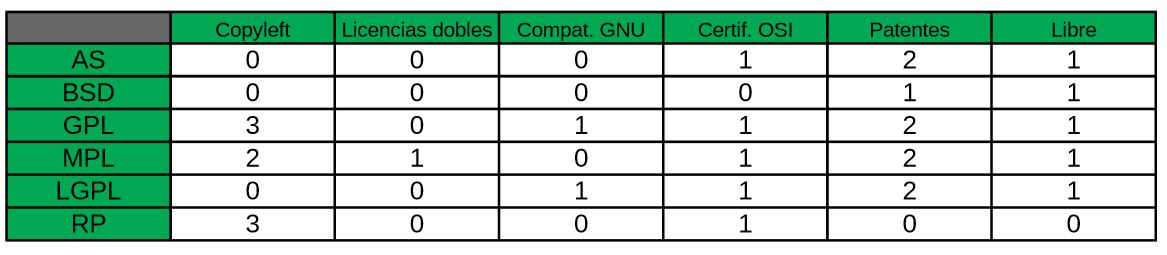
\includegraphics[scale=0.48]{1} 
	\caption{Rejilla de repertorio} \label{etiq}
\end{figure}

\begin{figure}[H] %con el [H] le obligamos a situar aquí la figura
	\centering
	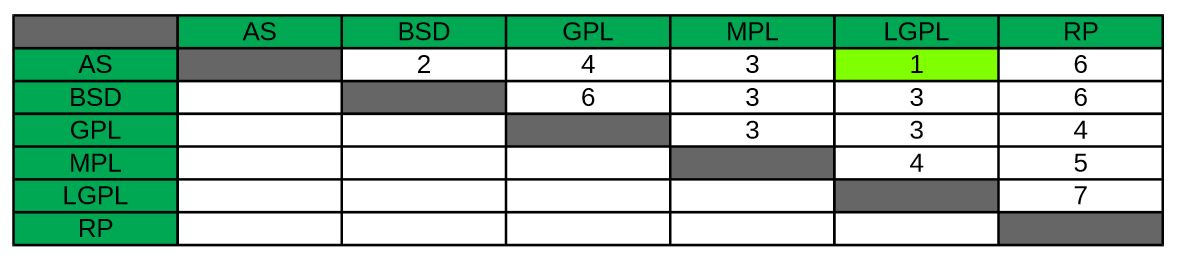
\includegraphics[scale=0.48]{2} 
	\caption{Rejilla de repertorio} \label{etiq}
\end{figure}

\begin{figure}[H] %con el [H] le obligamos a situar aquí la figura
	\centering
	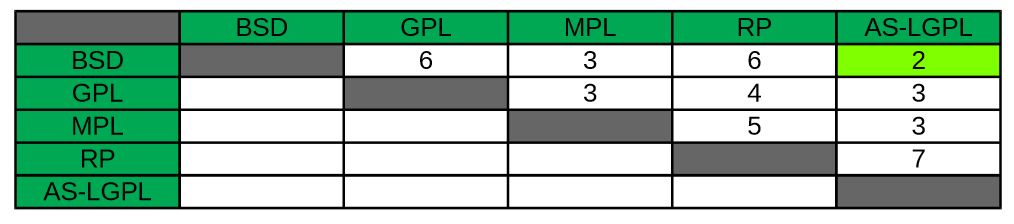
\includegraphics[scale=0.48]{3} 
	\caption{Rejilla de repertorio} \label{etiq}
\end{figure}

\begin{figure}[H] %con el [H] le obligamos a situar aquí la figura
	\centering
	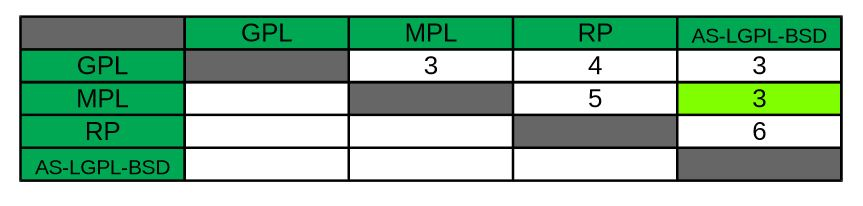
\includegraphics[scale=0.48]{4} 
	\caption{Rejilla de repertorio} \label{etiq}
\end{figure}

\begin{figure}[H] %con el [H] le obligamos a situar aquí la figura
	\centering
	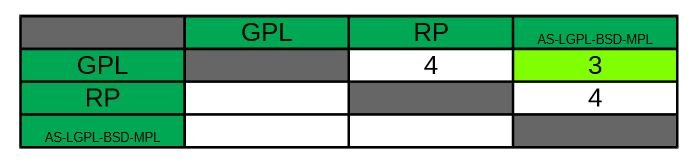
\includegraphics[scale=0.48]{5} 
	\caption{Rejilla de repertorio} \label{etiq}
\end{figure}

\begin{figure}[H] %con el [H] le obligamos a situar aquí la figura
	\centering
	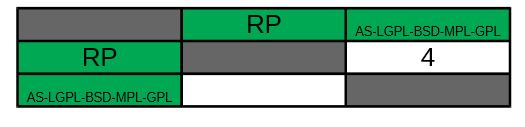
\includegraphics[scale=0.48]{6} 
	\caption{Rejilla de repertorio} \label{etiq}
\end{figure}

La siguiente figura es el árbol de decisión creado para la implementación del primer módulo:

\begin{figure}[H] %con el [H] le obligamos a situar aquí la figura
	\centering
	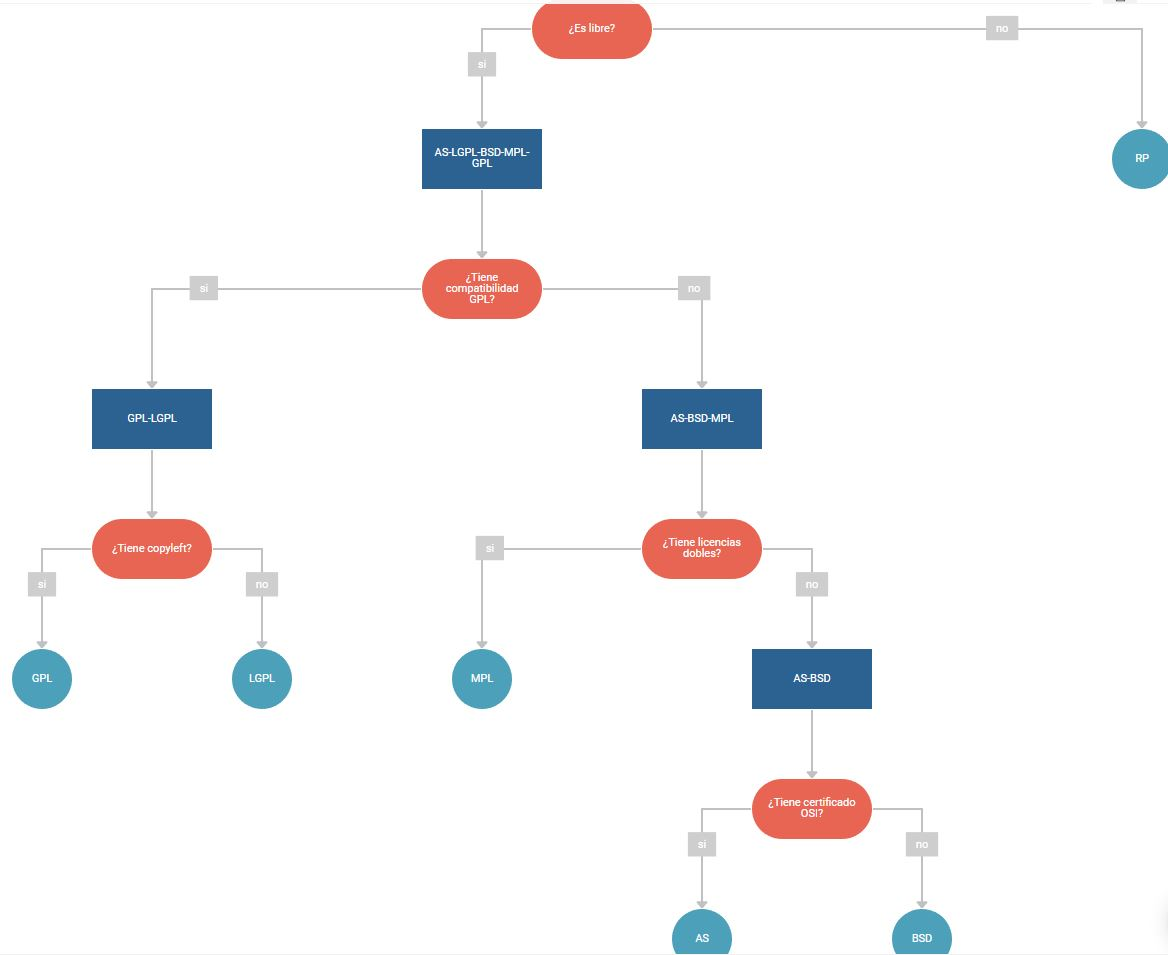
\includegraphics[scale=0.55]{7} 
	\caption{Árbol de decisión} \label{etiq}
\end{figure}

Con respecto a la obtención  de conocimiento en\textbf{ el segundo de los módulos} que era necesario implementar, el proceso fue exactamente igual, es decir, la consulta de compatibilidades entre licencias software la realicé en las mismas páginas web. Sin embargo el árbol de decisión aprendido fue gracias al fichero CTree.xls proporcionado por los profesores de la asignatura.
A continuación muestro el árbol de decisión obtenido modificando el fichero CTree.xls para que compare dos a dos todas las licencias, diciendo si son o no compatibles entre ellas y realice un profundo estudio mediante aprendizaje automático del árbol el cual nos contestará a la pregunta de ''¿qué características he de comprobar para saber si dos licencias son compatibles?'':

\begin{figure}[H] %con el [H] le obligamos a situar aquí la figura
	\centering
	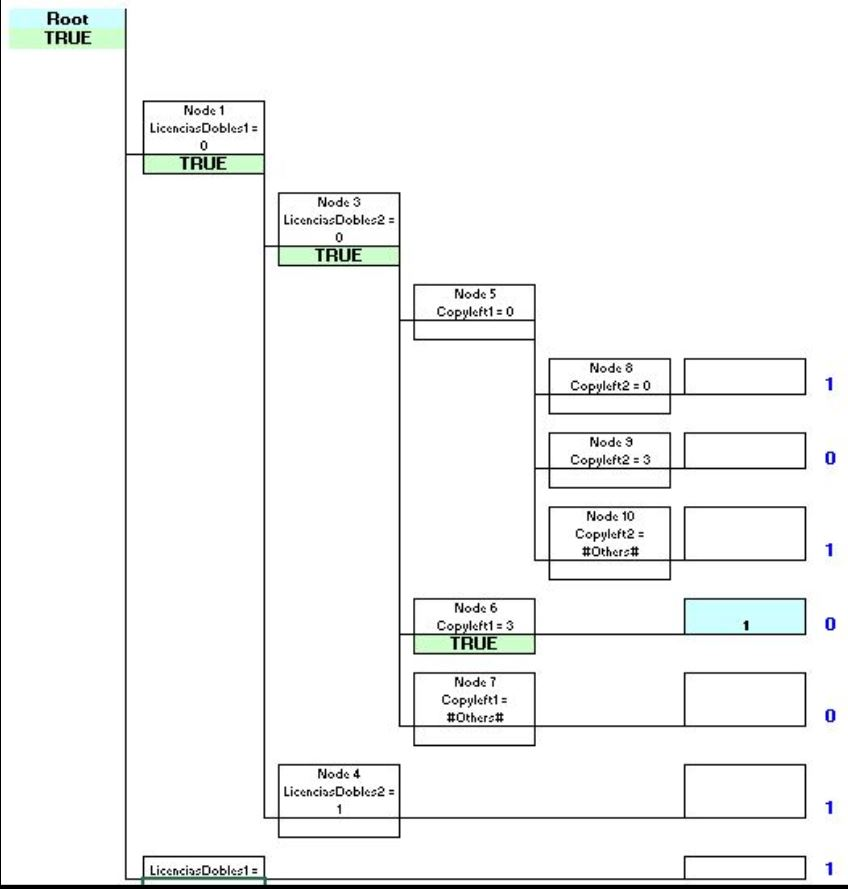
\includegraphics[scale=0.65]{8} 
	\caption{Árbol de decisión} \label{etiq}
\end{figure}

Como podemos observar con tan solo dos características podemos averiguar si dos de las licencias seleccionadas por el usuario son compatibles entre sí, todo gracias al árbol de decisión aprendido, como he mencionado antes.
\\

Con respecto al \textbf{módulo 3}, los datos manejados por el sistema (LOPD) han sido tomados de las páginas referenciadas en la guía de la práctica.
El apartado 3 de dicho módulo ha sido implementado siguiendo mi propio criterio a la hora de decidir cuales son los datos que nos proporcionan una identificación total o parcial de un individuo.
\newpage

\subsection{Procedimiento de validación y verificación del sistema.}


\begin{itemize}
	\item \textbf{Verificación}: me he encargado de comprobar que el sistema no posee ningún tipo de error semántico, lógico o estructural, de tal manera que no sufre bloqueos en bucles, ni existen reglas que nunca puedan llegar a darse, al mismo tiempo que tampoco existen variables que puedan tomar valores ilegales o no válidos.
	\item \textbf{Validación}: he hecho las veces de usuario, ejecutando cada una de las casuísticas exitentes en mi sistema y, comprobando la consistencia y robustez del mismo, al mismo tiempo que me he intentado asegurar de la certeza del conocimiento obtenido.
\end{itemize}



\section{Descripción del sistema desarrollado}

\subsection{Variables de entrada del problema}

Como variables de entrada de mi sistema distinguimos según el módulo que se ejecuta:
\begin{itemize}
	\item \textbf{Módulo 1}: Las variables de entrada se corresponden con las sucesivas contestaciones que el usuario responde a las cuestiones que el sistema proporciona a la hora de encaminarlo por la ruta adecuada del árbol de decisiones.
	\item \textbf{Módulo 2}: En este módulo las únicas variables de entrada son las dos licencias para las cuales se desea saber si son compatibles con las características que posee cada una o no.
	\item \textbf{Módulo 3}: Cada una de las preguntas generadas por el sistema en este módulo hacen que el usuario tenga que introducir unas cuantas variables de entrada. Estas son por ejemplo, los datos a utilizar, el tipo de organización que los usará, el uso que se les dará...
\end{itemize}


\subsection{Variables de salida del problema}

Como variables de entrada de mi sistema distinguimos según el módulo que se ejecuta:
\begin{itemize}
	\item \textbf{Módulo 1}: En este módulo la variable de salida se corresponde con la licencia adecuada para el usuario en cuestión.
	\item \textbf{Módulo 2}: Aquí la variable de salida es una respuesta a: ¿es compatible la licencia A con la licencia B? Además de la explicación asociada a la respuesta.
	\item \textbf{Módulo 3}: Las variables de salida son dos en este caso. La primera es una clasificación de los datos que el usuario ha decidido utilizar.
	La segunda es la respuesta a la pregunta: ¿con los datos escogidos podemos identificar total, parcial o de forma nula a un individuo?
\end{itemize}

\newpage

\subsection{Conocimiento global del sistema: hechos y relaciones iniciales}
A continuación comentaré los hechos y las relaciones creadas inicialmente para la ejecución de los distintos módulos.
\begin{itemize}
	\item \textbf{Módulo 1}
		\begin{itemize}
			\item tiposLicencias: establece para cada una de las características medidas, cuales son las licencias que la poseen.
			\item controlLicenciasEscogidas: nos permite mantener el control de lo que el usuario introduce por teclado y repetir las preguntas en caso de que se introduzca algo no válido.
		\end{itemize}
	\item \textbf{Módulo 2}
		\begin{itemize}
			\item caracteristicasLicencias: lista de cada una de las licencias con cada una de las características que tienen para conocerlas en las reglas y poder comparar las unas con las otras a la hora de conocer si son compatibles o no.
			\item valoresCopyleft: lista de los posibles valores que puede tomar la características copyleft en cada una de las licencias. Puede tomar los valores: noCopyleft, copyleftLimitado y copyleft.
			\item valoresLicenciasDobles: exactamente igual que el hecho anterior pero, con la característica "licenciasDobles" pudiendo tomar los valores: sinLicenciasDobles y conLicenciasDobles.
		\end{itemize}
	\item \textbf{Módulo 3}
		\begin{itemize}
			\item 
			\item identificacionDePersonas: hecho que ayuda en la resolución del apartado 3.3 de la práctica. En este hecho defino cuales (a mi parecer) son los datos que nos aportan una identificación total de un individuo, cuales son los que aportan una identificación parcial y cuales lo que aportan una identificación nula.
			\item tiposDatos: aquí definimos los "datos de carácter personal" proporcionados por la LOPD con cada uno de sus tipos asociados. Gracias a ello podemos realizar la impresión de los datos escogidos por el usuario y la clasificación de estos.
			\item tiposOrganizaciones: para el control de la introducción por teclado de los tipos de organizaciones que usarán los datos.
			\item tiposLugares:  para el control de la introducción por teclado de los lugares posibles donde operarán los datos.
			\item tiposUsos:  para el control de la introducción por teclado de los posibles usos que se le podrán dar a los datos.
			\item identificacionPersonas: deftemplate para asociar a cada dato el tipo de identificación que tiene.
		\end{itemize}
\end{itemize}

\subsection{Especificación de cada módulo}
	
A continuación paso a describir cada uno de los módulos implementados:
\begin{itemize}
	\item \textbf{Elección de licencia de software}:\\
		\begin{itemize}
			\item \textbf{Objetivo}: Descubrir al usuario, de las licencias disponibles en el sistema, cual es la más adecuada en función de los requisitos que este desee para su software.
			\item \textbf{Conocimiento utilizado}: El conocimiento usado es el obtenido mediante la rejilla de repertorio realizada a mano, la cual nos proporciona el árbol de decisión sobre el que guiar las ideas del usuario.
			\item \textbf{Conocimiento deducido}: El conocimiento deducido son las posibles licencias que pueden obtenerse y el por qué de las elecciones tomadas en cada una de las casuísticas posibles dadas por el sistema experto.
		\end{itemize}
	\item \textbf{Compatibilidades entre diferentes licencias software}\\
		\begin{itemize}
			\item \textbf{Objetivo}: Definir compatibilidades entre parejas de licencias (la del software que se está utilizando y la que se desea utilizar). El objetivo es informar al usuario de dichas compatibilidades.
			\item \textbf{Conocimiento utilizado}: El árbol de decisión creado, el cual nos conduce a saber cuales son las características que hemos de mirar para conocer de forma precisa si dos licencias de las que hay actualmente en la base de datos son compatibles o no.
			\item \textbf{Conocimiento deducido}: La propia compatibilidad entre licencias software a partir de dicho árbol
		\end{itemize}
	\item \textbf{Asesoramiento sobre ley de protección de datos}	\\
		\begin{itemize}
			\item \textbf{Objetivo}: Hacer conocer al usuario todo lo necesario acerca de la LOPD (Ley de protección de datos) para que este pueda actuar dentro del marco legal y los acuerdos preestablecidos, además de conocer los derechos ARCO a ejercer.
			\item \textbf{Conocimiento utilizado}: Información extraída de las fuentes de información proporcionadas en el guión de la asignatura. Dicha información son tanto los datos de carácter personal a utilizar, como los tipos de organización que usarán los datos, como los usos posibles que se les dará a estos, etc.
			\item \textbf{Conocimiento deducido}: En este caso el conocimiento deducido consiste en la clasificación de los tipos de datos que el usuario ha decidido utilizar en los distintos grupos de caracterización según la LOPD y, en segundo lugar, la inferencia proporcionada por el sistema de, si el conjunto de datos seleccionado por el usuario es suficiente como para identificar de forma total o parcial a un individuo.
		\end{itemize}
\end{itemize}



\subsection{Estructura de funcionamiento del esquema de razonamiento del sistema}

Como ya he comentado, el funcionamiento del sistema está esquematizado de manera bien clara en tres bloques o módulos:
\begin{enumerate}
	\item Elección de licencia software.
	\item Consulta de compatibilidades entre licencias.
	\item Asesoramiento sobre ley de protección de datos.
\end{enumerate}

Cada uno de estos módulos posee una serie de hechos y reglas propios los cuales le permiten llevar a cabo el objetivo con el que se pretende ayudar al usuario.
Para ejecutar o lanzar cada uno de los módulos, el usuario simplemente ha de elegir en el menú inicial creado para el sistema, cual de los tres bloques desea ejecutar, el 1, el 2 o el 3.\\
De esta manera, si ha introducido por teclado un 1, entonces el sistema lanzará el primer módulo con el fin de ayudar a dicho usuario en la elección de la licencia adecuada para su sistema software, y así sucesivamente para el resto de los módulos.



\subsection{Representación de los hechos utilizados por el sistema}
En este apartado me dispongo a formalizar la representación del conocimiento en cada uno de los hechos utilizados por el sistema
\begin{itemize}
	\item \textbf{Módulo 1}
	\begin{itemize}
		\item tiposLicencias: (<caracteristica> <licencia1> <licencia2>...)
		\item controlLicenciasEscogidas: (licenses <nombreLicencia1> <nombreLicencia2>...), (licenciaEscogida nombreInicial). De esta manera cuando el usuario introduce un nombre por teclado, nombreInicial ha de ser igual a alguna de las licenses definidas.
	\end{itemize}
	\item \textbf{Módulo 2}
	\begin{itemize}
		\item caracteristicasLicencias: (licencia <nombreLicencia> <caracteristica1> <caracteristica2>...)
		\item valoresCopyleft: (copy noCopyleft copyleftLimitado copyleft). (posibles valores que puede tomar copyLeft)
		\item valoresLicenciasDobles: (dobles sinLicenciasDobles conLicenciasDobles). (posibles valores que puede tomar licenciasDobles)
	\end{itemize}
	\item \textbf{Módulo 3}
	\begin{itemize}
		\item identificacionDePersonas: (dato\_identificacion <nivelIdentificacion> <dato>).
		\item tiposDatos: (tipoDato <tipo> <dato>).
		\item tiposOrganizaciones: (tiposOrganizacionesPosibles UD EP ODAP), (tipoOrganizacionEscogido AAAA). De manera que cuando el usuario introduzca el tipo de organización por teclado, esta ha de coincidir con una de las definidas.
		\item tiposLugares:  para el control de la introducción por teclado de los lugares posibles donde operarán los datos.(tiposLugaresPosibles asia europa oceania america africa), (lugarEscogido AAAA).
		De manera que cuando el usuario introduzca el lugar por teclado, este ha de coincidir con uno de los definidos.
		\item tiposUsos:  (tiposUsosDisponibles domestico negocios judiciales seguridad), (usoEscogido AAAA).
		De manera que cuando el usuario introduzca el uso deseado por teclado, este ha de coincidir con uno de los definidos. 
		\item identificacionPersonas: (field dato) (field tipoIdentificacion)
	\end{itemize}
\end{itemize}

\subsection{Reglas de cada uno de los módulos}

Estas son las reglas utilizadas (explicadas de manera general) para la resolución de cada uno de los módulos. Todas las reglas tienen implícito un control de errores mediante el cual el sistema se asegura de que el usuario solo pueda introducir términos con valores permitidos, lo que garantiza el buen funcionamiento del sistema.

\begin{itemize}
	\item \textbf{Módulo 1}:
		\begin{itemize}
			\item \textbf{licenciasDisponibles}: Impresión por pantalla de las licencias que hay disponibles en el sistema.
			\item \textbf{preguntaX}: realiza la pregunta X del árbol de decisión aprendido mediante la rejilla de repertorio.
			\item \textbf{aceptarAfirmacionX}: en caso de que el usuario responda afirmativamente se lanza una regla A.
			\item \textbf{aceptarNegacionX}: en caso de que el usuario responda de forma negativa se lanza otra regla B.
		\end{itemize}
	\item \textbf{Módulo 2}:
		\begin{itemize}
			\item \textbf{lecturaLicenciaX}: realiza la lectura por teclado de la licencia X (donde X es 1 o 2, ya que solo se comparan dos licencias) que el usuario quiera escoger.
			\item \textbf{ramaArbolDecisionX}: son las reglas que controlan cada una de las ramas existentes en el árbol de decisión creado por CTree.xls. Hay 2 reglas menos que ramas existentes, ya que hay 2 ramas en el árbol creado que, con el conocimiento que posee mi sistema nunca llegarían a ejecutarse, por tanto hay 5 ramas en total. Cada una de las reglas controla en los antecedentes lo que ha de ocurrir para avanzar por dicha rama, controlando como he dicho antes, las únicas dos características que son necesarias para saber si dos licencias son compatibles en mi sistem: copyleft y licencias dobles.
		\end{itemize}
	\item \textbf{Módulo 3}:
		\begin{itemize}
			\item \textbf{mostrarDatosManejables}: muestra la lista de datos que son manejables por el sistema, los propuestos por la LOPD como "datos personales".
			\item \textbf{escogerDatos}: regla que permite al usuario escoger los datos que desee de la lista anterior.
			\item \textbf{denegarContestacion}: en caso de que se equivoque no aserta el hecho con lo que haya introducido el usuario.
			\item \textbf{aceptarContestacion}: en caso de que se introdzca bien el dato, se aserta.
			\item \textbf{finRecogidaDatos}: cuando el usuario escribe "fin" por el teclado, se dejan de tomar datos de teclado y se procede a imprimirlos con sus correspondientes tipos.
			\item \textbf{impresionTiposEscogidos}: imprimimos por pantalla los datos escogidos con los tipos a los que pertenecen.
			\item \textbf{tiposDeOrganizaciones}: primera pregunta del apartado 2 del módulo 3. Se muestran las posibles organizaciones y se pide al usuario que introduzca la que desee.
			\item \textbf{lugaresGeograficosDisponibles}: segunda pregunta del apartado 2 del módulo 3. Se muestran los posibles lugares geográficos y se pide al usuario que introduzca el que desee.
			\item \textbf{usosDisponiblesDeDatos}: tercera pregunta del apartado 2 del módulo 3. Se muestran los posibles usos de los datos y se pide al usuario que introduzca el que desee.
			\item \textbf{insertarTiposIdentificacionsADatos}: se encarga de asertar cada dato introducido por el usuario con el tipo de identificación que posee.
			\item \textbf{determinarIdentificacionPersonaX}: hay en total 5 reglas de este estilo, las cuales se encargan de analizar los tipos de identificación que pueden darse con los datos que ha escogido por teclado el usuario del sistema. Estos son los 5 tipos de identificaciones:
			\begin{enumerate}
				\item Dos datos con tipo de identificación total, lo que nos da una identificación \textbf{total} del individuo.
				\item Dos datos con tipo de identificación parcial y uno con tipo de identificación \textbf{total}, lo que nos da una identificación total del individuo.
				\item Cuatro datos con tipo de identificación parcial, lo que nos da una identificación \textbf{total} del individuo.
				\item Tres datos con tipo de identificación parcial, lo que nos da una identificación \textbf{parcial} del individuo.
				\item Dos datoscon tipo de identificación parcial, lo que nos da una identificación \textbf{parcial} del individuo.
			\end{enumerate}
			\item \textbf{determinarNoIdentificacionPersona}: esta regla se lanza única y exclusivamente cuando no se lanza ninguna de las anteriores, lo cual ocurrirá cuando el usuario haya escogido tan solo datos con tipo de identificación nula o un solo dato con tipo de identificación parcial.
		\end{itemize}
\end{itemize}


\section{Uso del sistema}

Para la ejecución del sistema simplemente hay que ejecutar los siguientes comandos en CLIPS: 

\begin{enumerate}
	\item \textbf{(clear)}
	\item \textbf{(load p2.clp)}
	\item \textbf{(reset)}
	\item \textbf{(run)}
\end{enumerate}

Una vez realizado esto se mostrará el menú anteriormente comentado en el cual se da a elegir por el lanzamiento de uno de los tres módulos distintos exigidos en la práctica. Para elegir uno de estos habrá que pulsar las teclas 1, 2 o 3 en función del bloque que queramos ejecutar.\\

Por motivos de falta de tiempo durante estos últimos dias, me ha sido imposible avanzar en la práctica a partir del punto 3.4, es decir, no he podido realizar los puntos 4 y 5 del módulo 3 de la práctica.






















\end{document}
